\documentclass[journal,12pt,twocolumn]{IEEEtran}
\usepackage{amsmath}
\usepackage{calc}
\usepackage{enumerate}
\usepackage{amssymb}
\usepackage{graphicx}
\usepackage{listings}
\usepackage{setspace}
\usepackage{gensymb}
\usepackage{caption}
%\usepackage{multirow}
%\usepackage{multicolumn}
%\usepackage{subcaption}
%\doublespacing
\singlespacing
\usepackage{csvsimple}
\usepackage{amsmath}
\usepackage{multicol}
\usepackage{enumerate}
\usepackage{amssymb}
%\usepackage{graphicx}
\usepackage{newfloat}
%\usepackage{syntax}
\usepackage{listings}
\usepackage{iithtlc}
\usepackage{color}
\usepackage{tikz}
\usetikzlibrary{shapes,arrows}



%\usepackage{graphicx}
%\usepackage{amssymb}
%\usepackage{relsize}
%\usepackage[cmex10]{amsmath}
%\usepackage{mathtools}
%\usepackage{amsthm}
%\interdisplaylinepenalty=2500
%\savesymbol{iint}
%\usepackage{txfonts}
%\restoresymbol{TXF}{iint}
%\usepackage{wasysym}
\usepackage{amsthm}
\usepackage{mathrsfs}
\usepackage{txfonts}
\usepackage{stfloats}
\usepackage{cite}
\usepackage{cases}
\usepackage{mathtools}
\usepackage{caption}
\usepackage{enumerate}	
\usepackage{enumitem}
\usepackage{amsmath}
%\usepackage{xtab}
\usepackage{longtable}
\usepackage{multirow}
%\usepackage{algorithm}
%\usepackage{algpseudocode}
\usepackage{enumitem}
\usepackage{mathtools}
\usepackage{hyperref}
%\usepackage[framemethod=tikz]{mdframed}
\usepackage{listings}
    %\usepackage[latin1]{inputenc}                                 %%
    \usepackage{color}                                            %%
    \usepackage{array}                                            %%
    \usepackage{longtable}                                        %%
    \usepackage{calc}                                             %%
    \usepackage{multirow}                                         %%
    \usepackage{hhline}                                           %%
    \usepackage{ifthen}                                           %%
  %optionally (for landscape tables embedded in another document): %%
    \usepackage{lscape}     


\usepackage{url}
\def\UrlBreaks{\do\/\do-}


%\usepackage{stmaryrd}

\begin{document}
%\usepackage{wasysym}
%\newcounter{MYtempeqncnt}
%\renewcommand{\baselinestretch}{2}
\renewcommand\thesection{\arabic{section}}
\renewcommand\thesubsection{\thesection.\arabic{subsection}}
\renewcommand\thesubsubsection{\thesubsection.\arabic{subsubsection}}

\renewcommand\thesectiondis{\arabic{section}}
\renewcommand\thesubsectiondis{\thesectiondis.\arabic{subsection}}
\renewcommand\thesubsubsectiondis{\thesubsectiondis.\arabic{subsubsection}}

% correct bad hyphenation here
\hyphenation{op-tical net-works semi-conduc-tor}

%\lstset{
%language=C,
%frame=single, 
%breaklines=true
%}

%\lstset{
	%%basicstyle=\small\ttfamily\bfseries,
	%%numberstyle=\small\ttfamily,
	%language=Octave,
	%backgroundcolor=\color{white},
	%%frame=single,
	%%keywordstyle=\bfseries,
	%%breaklines=true,
	%%showstringspaces=false,
	%%xleftmargin=-10mm,
	%%aboveskip=-1mm,
	%%belowskip=0mm
%}

%\surroundwithmdframed[width=\columnwidth]{lstlisting}
\def\inputGnumericTable{}                                 %%
\lstset{
%language=C,
frame=single, 
breaklines=true,
columns=fullflexible
}

%
\tikzstyle{block} = [rectangle, draw,
    text width=3em, text centered, minimum height=3em]
\tikzstyle{sum} = [draw, circle, node distance=3cm]
\tikzstyle{input} = [coordinate]
\tikzstyle{output} = [coordinate]
\tikzstyle{pinstyle} = [pin edge={to-,thin,black}]

\theoremstyle{definition}
\newtheorem{theorem}{Theorem}[section]
\newtheorem{problem}{Problem}
\newtheorem{proposition}{Proposition}[section]
\newtheorem{lemma}{Lemma}[section]
\newtheorem{corollary}[theorem]{Corollary}
\newtheorem{example}{Example}[section]
\newtheorem{definition}{Definition}[section]
%\newtheorem{algorithm}{Algorithm}[section]
%\newtheorem{cor}{Corollary}
\newcommand{\BEQA}{\begin{eqnarray}}
\newcommand{\EEQA}{\end{eqnarray}}
\newcommand{\define}{\stackrel{\triangle}{=}}
\bibliographystyle{IEEEtran}
%\bibliographystyle{ieeetr}
\providecommand{\nCr}[2]{\,^{#1}C_{#2}} % nCr
\providecommand{\nPr}[2]{\,^{#1}P_{#2}} % nPr
\providecommand{\mbf}{\mathbf}
\providecommand{\pr}[1]{\ensuremath{\Pr\left(#1\right)}}
\providecommand{\qfunc}[1]{\ensuremath{Q\left(#1\right)}}
\providecommand{\sbrak}[1]{\ensuremath{{}\left[#1\right]}}
\providecommand{\lsbrak}[1]{\ensuremath{{}\left[#1\right.}}
\providecommand{\rsbrak}[1]{\ensuremath{{}\left.#1\right]}}
\providecommand{\brak}[1]{\ensuremath{\left(#1\right)}}
\providecommand{\lbrak}[1]{\ensuremath{\left(#1\right.}}
\providecommand{\rbrak}[1]{\ensuremath{\left.#1\right)}}
\providecommand{\cbrak}[1]{\ensuremath{\left\{#1\right\}}}
\providecommand{\lcbrak}[1]{\ensuremath{\left\{#1\right.}}
\providecommand{\rcbrak}[1]{\ensuremath{\left.#1\right\}}}
\theoremstyle{remark}
\newtheorem{rem}{Remark}
\newcommand{\sgn}{\mathop{\mathrm{sgn}}}
\providecommand{\abs}[1]{\left\vert#1\right\vert}
\providecommand{\res}[1]{\Res\displaylimits_{#1}} 
\providecommand{\norm}[1]{\left\Vert#1\right\Vert}
\providecommand{\mtx}[1]{\mathbf{#1}}
\providecommand{\mean}[1]{E\left[ #1 \right]}
\providecommand{\fourier}{\overset{\mathcal{F}}{ \rightleftharpoons}}
%\providecommand{\hilbert}{\overset{\mathcal{H}}{ \rightleftharpoons}}
\providecommand{\system}{\overset{\mathcal{H}}{ \longleftrightarrow}}
	%\newcommand{\solution}[2]{\textbf{Solution:}{#1}}
\newcommand{\solution}{\noindent \textbf{Solution: }}
\newcommand{\myvec}[1]{\ensuremath{\begin{pmatrix}#1\end{pmatrix}}}
\providecommand{\dec}[2]{\ensuremath{\overset{#1}{\underset{#2}{\gtrless}}}}
\DeclarePairedDelimiter{\ceil}{\lceil}{\rceil}
%\numberwithin{equation}{section}
%\numberwithin{problem}{subsection}
%\numberwithin{definition}{subsection}
\makeatletter
\@addtoreset{figure}{section}
\makeatother
\let\StandardTheFigure\thefigure
%\renewcommand{\thefigure}{\theproblem.\arabic{figure}}
\renewcommand{\thefigure}{\thesection}
%\numberwithin{figure}{subsection}
%\numberwithin{equation}{subsection}
%\numberwithin{equation}{section}
%\numberwithin{equation}{problem}
%\numberwithin{problem}{subsection}
\numberwithin{problem}{section}
%%\numberwithin{definition}{subsection}
%\makeatletter
%\@addtoreset{figure}{problem}
%\makeatother
\makeatletter
\@addtoreset{table}{section}
\makeatother
\let\StandardTheFigure\thefigure
\let\StandardTheTable\thetable
\let\vec\mathbf
\numberwithin{equation}{section}%language=C,
\providecommand{\pr}[1]{\ensuremath{\Pr\left(#1\right)}}
\providecommand{\sbrak}[1]{\ensuremath{{}\left[#1\right]}}
\providecommand{\brak}[1]{\ensuremath{\left(#1\right)}}
\title{PDF and CDF of uniform and gaussian distributions}
\author{Kushagra Gupta}

\date{}


\maketitle
\section{Uniform Random Numbers}
Let $U$ be a uniform random variable between 0 and 1.
\begin{enumerate}[label=\thesection.\arabic*,ref=\thesection.\theenumi]
    \item\textbf{Question:} Generate $10^6$ samples of $U$ using a C program and save into a file called uni.dat .\\
Download the following files and execute the  C program.
        \begin{lstlisting}
wget https://github.com/gadepall/probability/raw/master/manual/codes/exrand.c
wget https://github.com/gadepall/probability/raw/master/manual/codes/coeffs.h
\end{lstlisting}
\textbf{Solution:}\\
\texttt{\$ gcc exrand.c -lm}\\
\texttt{\$ ./a.out}\\
Note: The flag \texttt{-lm} is to tell gcc to include the math library.\\ 
This code creates the file "uni.dat" which contains random data points for a uniform distribution.





\item\textbf{Question:} Load the uni.dat file into python and plot the empirical CDF of $U$ using the samples in uni.dat. The CDF is defined as
\begin{align}
F_{U}(x) = \pr{U \le x}
\end{align}
Download the follwing file for plotting cdf.
\begin{lstlisting}
wget https://github.com/gadepall/probability/raw/master/manual/codes/cdf_plot.py
\end{lstlisting}
\textbf{Solution:}\\
\texttt{\$ python3 cdf\_plot.py}\\
This plots the numerical part of fig.1



\item\textbf{Question:} Find a  theoretical expression for $F_{U}(x)$.\\
\textbf{Solution:} Given $U$ is a uniformly distributed random variable over the interval $(0, 1)$, we have the density function $p_U(x)$:

\begin{align}
	p_U(x) =
            \begin{cases}
    		1, & x \in (0, 1) \\
    		0, & otherwise
	    \end{cases}
    	\label{eq:PDF}
\end{align}

We know that,
\begin{align}
    F_U(x) = \int_{-\infty}^{x} p_U(x) \,dx
    \label{eq:Relation}
\end{align}

\noindent $\therefore$ We have the following expression for $F_U(x)$:
\begin{align}
    F_U(x) =
	    \begin{cases}
	    	0, & x \in (-\infty, 0) \\
  	    	x, & x \in (0, 1) \\
    		1, & x \in (1, \infty)\\
            \end{cases}
\end{align}


\item\textbf{Question:} The mean of $U$ is defined as
%
\begin{align}
E\sbrak{U} = \frac{1}{N}\sum_{i=1}^{N}U_i
\end{align}
%
and its variance as
%
\begin{align}
\text{var}\sbrak{U} = E\sbrak{U- E\sbrak{U}}^2 
\end{align}
Write a C program to  find the mean and variance of $U$.\\ 


\noindent \textbf{Solution:}\\
 \begin{lstlisting}
using ./code/exrand.c, we get the variance for the uniform distribution as 0.083301 and mean as 0.500007}
    \end{lstlisting}
    \begin{align}
    \text{We know that }&E(U) = \int _ {-\infty} ^ {\infty} {x d(F_U(x))}\\
    \implies &E(U) = \int _ {0} ^ {1} {x dx}\\
    \implies &E(U) = 0.5
\end{align}

\begin{align}
    &E(U^1) = \int _ {- \infty} ^ {\infty} {x^2 d(F_u(x))} \\
    \implies &E(U^2) = \int _ {0} ^ {1} {x^2 dx} \\
    \therefore &E(U^2) = \frac{1}{3}
\end{align}

We know that
\begin{align}
    &var(U) = E(U^2) - (E(U))^2 \\
    \implies&var(U) = \frac{1}{3} - \frac{1}{4} \\
    \therefore &var(U) = \frac{1}{12} = 0.0825
\end{align}
\begin{figure}[!ht]
\centering
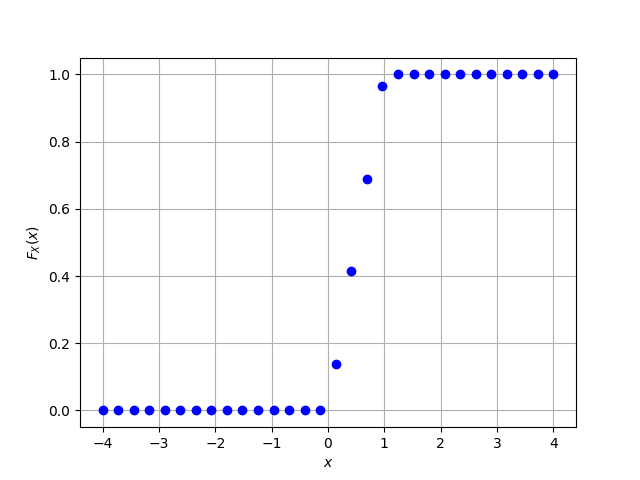
\includegraphics[width=\columnwidth]{./figs/Figure_Q1.png}
\caption{The CDF of $U$}
\label{fig: uniform distribution}
\end{figure}


Code command are as follows:\\
\texttt{\$ gcc exrand.c -lm}\\
\texttt{\$ ./a.out}\\
Note: The flag \texttt{-lm} is to tell gcc to include the math library.\\ 

   
\item\textbf{Question:}Verify your result theoretically given that
%
    \begin{align}
E\sbrak{U^k} = \int_{-\infty}^{\infty}x^kdF_{U}(x)
    \end{align}We are given that
\begin{align}
            &E[U^k] = \int^{\infty}_{-\infty} x^k dF_U(x)\\
    \implies&E[U^k] = \int^{\infty}_{-\infty} x^k p_U(x) \,dx		\label{eq: Expected}
\end{align}
We know that mean $\mu$ is given by $E(U)$.\\ Hence,

\begin{align}
    \mu &= \int_{-\infty}^{\infty} x p_U(x) \,dx\label{eq:Relation_1}\\
		\mu &= \int_{0}^{1} x \,dx \\
		&= \frac{x^2}{2} \big|^{1}_{0} \\
		&= \frac{1}{2} 	\label{eq: Mean}
\end{align}
\begin{align}
    var(U) = E((U - E(U))^2)
\end{align}
This can also be represented as
\begin{align}
		var(U) &= E(U^2 - 2E(U)U + (E(U))^2) \\
		&= E(U^2) - 2(E(U))^2 + (E(U))^2 \\
		&= E(U^2) - (E(U))^2
		\label{eq: Relation_2}
\end{align}
We can evaluate $E(U^2)$ using \eqref{eq: Expected} as:
	
\begin{align}
    	E(U^2) &= \int_{-\infty}^{\infty} x^2 p_U(x) \,dx \\
    	&= \int_{0}^{1} x^2 \,dx \\
    	&= \frac{x^3}{3} \big|^{1}_{0} \\
    	&= \frac{1}{3}
\end{align}

    Using \eqref{eq: Mean} and \eqref{eq: Relation_2} we have
\begin{align}
    	var(U) = \frac{1}{3} - \frac{1}{4} = \frac{1}{12}
\end{align}
\end{enumerate}
\section{Central Limit Theorem}
\begin{enumerate}[label=\thesection.\arabic*
,ref=\thesection.\theenumi]
        \item\textbf{Question:} Generate $10^6$ samples of the random variable\\
%
\begin{align}
X = \sum_{i=1}^{12}U_i -6
\end{align}
%
using a C program, where $U_i, i = 1,2,\dots, 12$ are  a set of independent uniform random variables between 0 and 1
and save in a file called gau.dat\\

\noindent \textbf{Solution:}
Code command are as follows:\\
\texttt{\$ gcc exrand.c -lm}\\
\texttt{\$ ./a.out}\\
Note: The flag \texttt{-lm} is to tell gcc to include the math library.\\
Note: The flag \texttt{-lm} is to tell gcc to include the math library.\\ 
This code creates the file "gau.dat" which contains random data points for a uniform distribution.




\item Download the follwing file for plotting cdf.
\begin{lstlisting}
wget https://github.com/gadepall/probability/raw/master/manual/codes/cdf_plot.py
\end{lstlisting}
\textbf{Solution:}\\
Code command are as follows:\\
\texttt{\$ python3 cdf\_plot.py}\\
This plots figure 2\\
\begin{figure}[!ht]
\centering
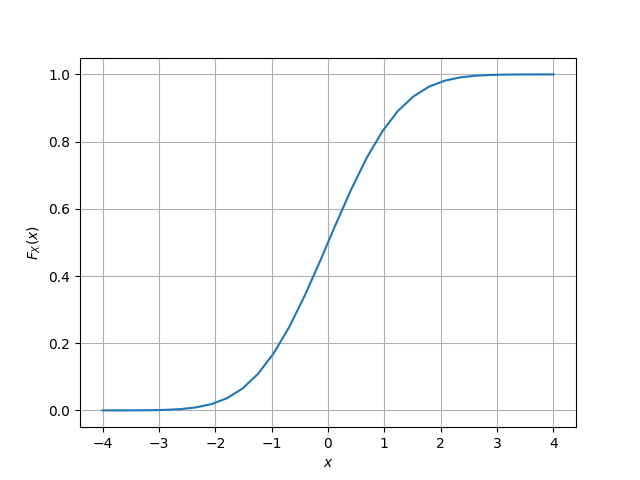
\includegraphics[width=\columnwidth]{./figs/Figure_2.png}
    \caption{The CDF of $X$}
\label{fig:gauss_X}
\end{figure}\\



The properties of CDF are:
    \begin{enumerate}
	\item The CDF never decreases (cumulative)
	\item $\lim_{x \to -\infty}F_X(x) = 0$
	\item $\lim_{x \to \infty}F_X(x) = 1$
    \end{enumerate}

\item\textbf{Question:}
Load gau.dat in python and plot the empirical PDF of $X$ using the samples in gau.dat. The PDF of $X$ is defined as
\begin{align}
p_{X}(x) = \frac{d}{dx}F_{X}(x)
\end{align}
\noindent \textbf{Solution:}\\

\noindent Code command are as follows:\\
\texttt{\$ python3 pdf\_plot.py}\\
This plots the figure 3.

\begin{figure}[!ht]
\centering
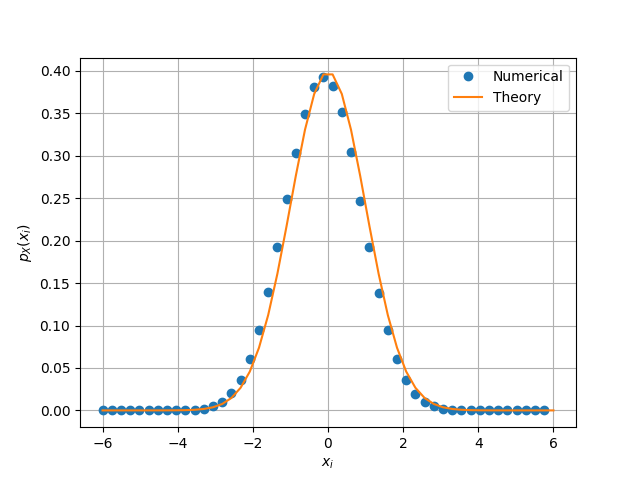
\includegraphics[width=\columnwidth]{./figs/Figure_3.png}
\caption{The PDF of $X$}
\label{fig:PDF_X}
\end{figure}




\item\textbf{Question: } Find the mean and variance of $X$ by writing a C program.\\
\noindent \textbf{Solution: }\\
\begin{lstlisting}
    using code ./code/exrand.c, we get the mean as 0.000326 and variance as 0.000906.
\end{lstlisting}


\item\textbf{Question: }Given that\\ 
\begin{align}
p_{X}(x) = \frac{1}{\sqrt{2\pi}}\exp\brak{-\frac{x^2}{2}}, -\infty < x < \infty,
\end{align}
repeat the above exercise theoretically.\\
\noindent \textbf{Solution: :}\\
For random variable $X$, we have been given the density function as follows
    \begin{align}
        &p_X(x) = \frac{1}{\sqrt{2\pi}}\exp{\frac{-x^2}{2}}\\
    \end{align}
For finding $\mu$,
\begin{align}
    \mu &= \int _ {- \infty} ^ {\infty} {x . p_X(x) dx} \\
    &= \int _ {- \infty} ^ {\infty} {x . \frac{1}{\sqrt{2 \pi}} e^{-x^2 / 2} dx}
\end{align}

As $x . p_X(x)$ is an odd function the above integral is $0$, therefore $\mu = 0$

For finding the variance $var$,
\begin{align}
    var &= E(X^2) \\
    &= \int _ {- \infty} ^ {\infty} {x^2 . \frac{1}{\sqrt{2 \pi}} e^{-x^2 / 2} dx} \\
    \text{let\,\,} x^2 &= 2t \\
    \implies var &= \int _ {- \infty} ^ {\infty} {\sqrt{2t} . \frac{1}{\sqrt{2\pi}} e^{-t} dt} \\
    &= \frac{2}{\sqrt{\pi}} \Gamma \left(\frac{3}{2}\right) \\
    \implies var &= 1
\end{align}
\item Theoritical expression of CDF in terms of Q function is \\
    \begin{align}
    Q_X(x) &= \int_x ^{\infty} \frac{1}{\sqrt{2\pi}} e^{\frac{-x^2}{2}} dx \\
      &= \frac{\text{erfc}(\frac{x}{\sqrt{2}})}{2}
   \end{align}
The CDF is then:
\begin{align}
    F_X(x) &= 1 - Q_X(x) \\
    &= 1 - \frac{\text{erfc}(\frac{x}{\sqrt{2}})}{2}
\end{align}
\end{enumerate}
\section{From Uniform to Other}

\begin{enumerate}[label=\thesection.\arabic*
,ref=\thesection.\theenumi]
\item\textbf{Question:}Generate samples of\\
%
\begin{align}
V = -2\ln\brak{1-U}
\end{align}
\noindent \textbf{Solution: }\\
Code command are as follows:\\
\texttt{\$ python3 cdf\_plot.py}\\
This plots figure 4\\
\begin{figure}[!ht]
\centering
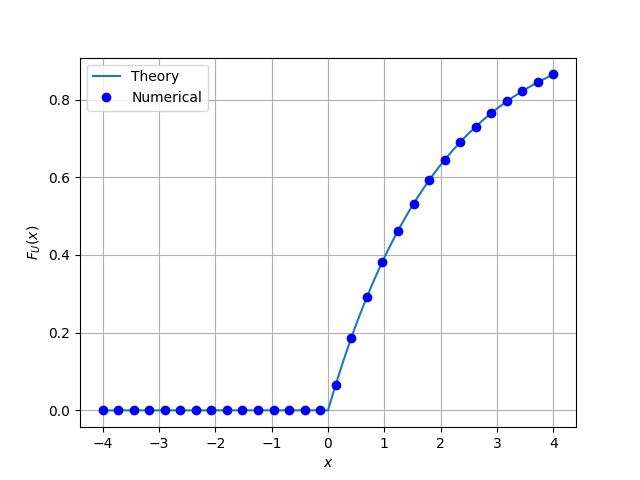
\includegraphics[width=\columnwidth]{./figs/Figure_Q4.png}
\caption{The CDF of $V$}
\label{fig:CDF_V}
\end{figure}





\item\textbf{Question:}
Find a theoretical expression for $F_V(x)$.

\noindent \textbf{Solution:}\\We have been given that random variable $V$ is a function of the random variable $U$ as follows:
\begin{align}
    V = -2\ln{(1 - U)}
\end{align}
	Note that the obtained distribution function (CDF) for random variable $U$ is:
\begin{align}
    	F_U(x) =
	\begin{cases}
		0, & x \in (-\infty, 0) \\
		x, & x \in (0, 1) \\
		1, & x \in (1, \infty)
	\end{cases}
\end{align}
We know for any random variable $X$
\begin{align}
    F_X(x) = \Pr(X \leq x)
\end{align}
	Hence, we can write:
\begin{align}
	F_V(x) &= \Pr(V \leq x) \\
	&= \Pr(-2\ln{(1 - U)} \leq x)\\
	&= \Pr(U \leq 1 - \exp{\frac{-x}{2}})\\
	&= F_U(1 - \exp{\frac{-x}{2}})
\end{align}
Note that the function $f(x) = 1 - \exp{\frac{-x}{2}}$ follows:
\begin{align}
    f(x) \in
	\begin{cases}
	    {0}, & x \in (-\infty, 0) \\
	    (0, 1) & x \in (0, \infty)
	\end{cases}
\end{align}
Hence we can write
\begin{align}
	F_V(x) =
	\begin{cases}
	    0, & x \in (-\infty, 0) \\
	    1 - \exp{\frac{-x}{2}}, & x \in (0, \infty)
    	\end{cases}
\end{align}

\end{enumerate}
\section{Triangular Distribution}
\begin{enumerate}[label=\thesection.\arabic*
,ref=\thesection.\theenumi]
        \item\textbf{Question:} Generate
        \begin{align}
            T = U_1 + U_2
        \end{align}
        \textbf{Solution:}\\
\texttt{\$ gcc exrand.c -lm}\\
\texttt{\$ ./a.out}\\
Note: The flag \texttt{-lm} is to tell gcc to include the math library.\\ 
This code creates the file "tri.dat" which contains random data points for a triangular distribution.
\item\textbf{Question: } Find the CDF of T\\
    \textbf{Solution: }\\
Code command are as follows:\\
\texttt{\$ python3 cdf\_plot.py}\\
This plots figure 5\\e
\begin{figure}[!ht]
\centering
\includegraphics[width=\columnwidth]{./figs/tri_cdf.png}
\caption{CDF of $T$}
\label{fig:CDF_T}
\end{figure}


\item\textbf{Question: } Find the PDF of T\\
    \textbf{Solution: }\\
Code command are as follows:\\
\texttt{\$ python3 pdf\_plot.py}\\
This plots figure 6\\
\begin{figure}[!ht]
\centering
\includegraphics[width=\columnwidth]{./figs/tri_pdf.png}
\caption{PDF of $T$}
\label{fig:PDF_T}
\end{figure}


\item\textbf{Question: } Find the theoritical expressions for the PDF and CDF of T.\\
    \textbf{Solution: }\\
    \begin{align}
    T = U_1 + U_2
\end{align}
where T, $U_1$ and $U_2$ are random variables, we have:
\begin{align}
    p_T(t) &= (p_{U_1} * p_{U_2})(t) \\
\end{align}
        Here, $p_{U_1}(t) = p_{U_2}(t) = p_U(t) $
\begin{align}
    p_T(t) &= \int _{-\infty} ^{\infty} p_U(\tau) p_U(t-\tau) d\tau \\
\end{align}
When $t < 0$ and $t > 2$ , the integral evaluates to $0$. When $0 < t < 1$:
\begin{align}
    p_T(t)  &= \int _0 ^1 p_U(t-\tau) d\tau \\
    &= \int _0 ^t p_U(t-\tau) d\tau \\
    &= t
\end{align}
when $ 1 < t < 2$:
\begin{align}
    p_T(t) &= \int _{t-1} ^1 p_U(t-\tau) d\tau \\
    &= 2-t
\end{align}
Therefore, we have:
\begin{align}
    p_T(x) =
    \begin{cases}
        x, & x \in (0,1) \\
        2-x, & x \in (1, 2) \\
        0, & otherwise
    \end{cases}
\end{align}
To find the CDF, we use:
\begin{align}
    F_T(x) = \int _{-\infty} ^x p_T(t) dt
\end{align}
We get:
\begin{align}
    F_T(x) =
    \begin{cases}
        0, & x \in (-\infty,0) \\
        \frac{x^2}{2}, & x \in (0,1) \\
        -\frac{x^2}{2} + 2x - 1, & x \in (1, 2) \\
        1, & x \in (2,\infty)
    \end{cases}
\end{align}
\item\textbf{Question: }Verify your results through a plot.\\
    \textbf{Solution: }\\
Code commands are as follows:\\
\texttt{\$ python3 cdf\_plot.py}\\
\texttt{\$ python3 pdf\_plot.py}\\
This plots figure 7 and 8\\
\begin{figure}[!ht]
\centering
\includegraphics[width=\columnwidth]{./figs/tri_cdf_sim.png}
\caption{CDF sim of $T$}
\label{fig:CDF_T_sim}
\end{figure}
\begin{figure}[!ht]
\centering
\includegraphics[width=\columnwidth]{./figs/tri_pdf_sim.png}
\caption{PDF sim of $T$}
\label{fig:PDF_T_sim}
\end{figure}







\end{enumerate}

\end{document}
